\section{Proofs}
\subsection{Theorem \ref{thm:projection}}\label{app:projection}
Consider the unique (up to symmetry) piece-wise affine map $T$ deforming $\Prism$ into a reference prism $\hat\Prism = \{u,v \geq 0|u+v \leq 1\} \times [-1,1]$, identifying the bottom surface of $\hat\Prism$ as $z=-1$, middle surface as $z=0$, and top surface as $z=1$.
Let $T_{\Tet}$ be the affine map mapping tetrahedron $\Tet$ to the reference prism.
Since the volume of all $\Tet$ is positive by assumption, the map $T$ is bijective and orientation preserving. 
In particular, $T$ transforms $\V(p)$ to the const vector $e_z = (0,0,1)$ since the edges of the prism are mapped to axis aligned edges of the reference prism. The projection operator $\P(p)$ can thus be equivalently defined as $\P(p) = T^{-1}(\P_z(T(p)))$, where $\P_z$ is the projection over the $z$-axis in the reference prism. 
$\P_z$ is bijective if the piecewise linear mesh intersecting $\Prism$ is composed of triangles with positive area (and the boundaries are mapped to the boundaries) \cite{lipman2014bijective}, after being mapped to the reference $\Prism$ and projected by $\P_z$. In the reference domain, having positive area after projection (with a fixed boundary) is equivalent to that the dot product between the projection direction and the normal of every face is positive. In the top half of $\Prism$, $\P_z$ is bijective if for every point $T(p), p \in f$ $T(n_p)\cdot [0,0,1] = T(n_p) \cdot T(\V(p)) > 0$  which holds since $ n_p \cdot \V(p) > 0$ (from the definition of section) and the fact that $T$ is orientation preserving and thus not changing the sign of the dot product.

%%%%%%%%%%%%%%%%%%%%%%%%%%%%%%%%%%%%%%%%%%
%%%%%%%%%%%%%%%%%%%%%%%%%%%%%%%%%%%%%%%%%%
%%%%%%%%%%%%%%%%%%%%%%%%%%%%%%%%%%%%%%%%%%
%%%%%%%%%%%%%%%%%%%%%%%%%%%%%%%%%%%%%%%%%%
%%%%%%%%%%%%%%%%%%%%%%%%%%%%%%%%%%%%%%%%%%
\subsection{Proposition \ref{thm:I1}}\label{app:I1}
%Let $\T$ be a triangle mesh without singularities and $\N$ be a displacement field satisfying $\mathbf{C} \N_i > 0$ for every vertex $v_i$ of $\T$. Then there exist a strictly positive per-vertex \emph{thickness} $\delta_i$ such that the shell created by displacing every vertex $v_i$ by $\delta_i \N_i$, to obtain the shell vertex $t_i$, and symmetrically for the bottom part, satisfies invariant I1. 

For simplicity, we will show that a uniform lower bound $\delta$ for all vertices exists. By consider a triangle of $T$, extruded over the displacement field $\N$, we obtain a generalized half prism with six vertices
$0$, $e_1$, $e_2$, $\delta n_0$, $e_1$ + $\delta n_1$, $e_2 + \delta$ $n_2$, with $\delta$ a positive constant. The indices of the tetrahedra are:
% \begin{tabular}{llll}
% 0 &2& 3& 4\\
% 0 &3& 4& 5\\
% 0 &1& 5& 3\\
% 0 &1& 2& 3\\
% 1 &2& 3& 4\\
% 0 &1& 2& 4\\
% 0 &1& 5& 4\\
% 1 &3& 4& 5\\
% 1 &2& 3& 5\\
% 0 &2& 5& 4\\
% 0 &1& 2& 5\\
% 2 &3& 4& 5\\
% \end{tabular}

(0 ,2, 3, 4), 
(0 ,3, 4, 5), 
(0 ,1, 5, 3), 
(0 ,1, 2, 3), 
(1 ,2, 3, 4), 
(0 ,1, 2, 4), 
(0 ,1, 5, 4), 
(1 ,3, 4, 5), 
(1 ,2, 3, 5), 
(0 ,2, 5, 4), 
(0 ,1, 2, 5), 
(2 ,3, 4, 5). 

For a sufficiently small $\delta$, the linear term will dominate the higher power of $\delta$, which we omit. 
The dominant volume terms are listed in the following table: ($e_{ij} := e_j - e_i$)

\vspace{1em}
{
% \begin{table}[t]
\footnotesize
%     \centering
    {
\begin{tabular}{|l|l|l|}
\hline
(0 ,2, 3, 4)&\text{vol1}$( 0,e_2,\delta  n_0,e_1 + \delta  n_1)           $&$ \delta \langle e_2,n_0,e_1\rangle$\\             
(0 ,3, 4, 5)&\text{vol2}$( 0,\delta  n_0,e_1 + \delta  n_1,e_2 + \delta n_2)   $&$ \delta \langle n_0,e_1,e_2\rangle $\\
(0 ,1, 5, 3)&\text{vol3}$( 0,e_1,e_2 + \delta n_2,\delta  n_0)            $&$ \delta \,\langle e_1,e_2,n_0\rangle  $\\
(0 ,1, 2, 3)&\text{vol4}$( 0,e_1,e_2,\delta  n_0)                    $&$ \delta \langle e_1,e_2,n_0\rangle                           $\\
(1 ,2, 3, 4)&\text{vol5}$( e_1,e_2,\delta  n_0,e_1 + \delta  n_1)         $&$ \langle e_{12}, \delta  n_0 - e_1, \delta n_1\rangle            $\\ 
&& $=\delta \langle e_2, -e_1, n_1\rangle     $\\
(0 ,1, 2, 4)&\text{vol6}$( 0,e_1,e_2,e_1 + \delta  n_1)             $&$ \delta \langle e_1,e_2,n_1\rangle                             $\\
(0 ,1, 5, 4)&\text{vol7}$( 0,e_1,e_2 + \delta n_2,e_1 + \delta  n_1)     $&$ \langle e_1,e_2 + \delta n_2, \delta  n_1\rangle                  $\\ 
&&$ =\delta \langle e_1,e_2,n_1\rangle                                           $\\
(1 ,3, 4, 5)&\text{vol8}$( e_1,\delta  n_0,e_1 + \delta  n_1,e_2 + \delta n_2) $&$ \delta \langle \delta  n_0 -e_1, n_1, e_{12} + \delta n_2\rangle    $\\ 
&&$ = \delta \langle -e_1, n_1, e_2\rangle                                   $\\
(1 ,2, 3, 5)&\text{vol9}$( e_1,e_2,\delta  n_0,e_2 + \delta n_2)          $&$ \langle e_{12}, \delta  n_0 - e_1, e_{12} + \delta n_2 \rangle $\\
&&$ =\delta \langle e_{12}, \delta  n_0 - e_1, n_2\rangle $\\
&&$ =\delta \langle e_2, - e_1, n_2\rangle $\\
(0 ,2, 5, 4)&\text{vol10}$( 0,e_2,e_2 + \delta n_2,e_1 + \delta  n_1)     $&$ \delta \langle e_2, n_2, e_1\rangle$ \\
(0 ,1, 2, 5)& \text{vol11}$( 0,e_1,e_2,e_2 + \delta n_2)$
                                                  &$ \delta \langle e_1,e_2,n_2\rangle $\\
(2, 3, 4, 5)&\text{vol12}$( e_2,\delta  n_0,e_1 + \delta  n_1,e_2 + \delta n_2) $&$ \langle \delta  n_0 - e_2, \delta  n_1-e_{12}, \delta  n_2\rangle      $\\
&&$ =\delta \langle - e_2, e_1, n_2\rangle$
                                                  \\
                                                  \hline
\end{tabular}}
% \end{table}
\vspace{1em}
}


For all the 12 tetrahedra the linear term is multiplied by a determinant containing the edges of the prism. We check directly that all these determinants are positive due to the assumption that $\mathbf{C} \N_i > 0$.

%%%%%%%%%%%%%%%%%%%%%%%%%%%%%%%%%%%%%%%%%%%%%%%%%%%%%%%%%%%%%%%%
%%%%%%%%%%%%%%%%%%%%%%%%%%%%%%%%%%%%%%%%%%%%%%%%%%%%%%%%%%%%%%%%
%%%%%%%%%%%%%%%%%%%%%%%%%%%%%%%%%%%%%%%%%%%%%%%%%%%%%%%%%%%%%%%%
\subsection{Theorem \ref{thm:thickness}}
\label{app:thickness}
%A valid shell $\S$ with respect to a section $\T$ always admits a strictly positive per-vertex thickness $\delta$.
% a shell with positive thickness exists that satisfies I1 and I2.

Consider a ball around a point $p$ of the middle face $M$ of the prism.  
If the radius $r(p) > 0$ is sufficiently small, it contains, at most, a single vertex of $M$, and parts of incident  faces. As $M$ is compact, there is a minimal value of $r$ on $M$, and it is positive. 
The line along the normal, passing through $v$, intersects incident faces at $v$ so it cannot intersect them at any other point. Thus, the top and bottom prism vertices can be obtained by displacing $V$ by $r$ in either direction along the normal. 
Consider the $r$-neighborhood of the $M$, i.e. the union of all balls of radius $r$ centered at 
points of $M$. This is a convex set, containing only $M$ and parts of vertex-adjacent faces. 
All top and bottom prism vertices are in this set. Thus tetrahedra connecting these vertices are also in the set, i.e., complete prisms. The fact that tetrahedra are nondegenerate is established in Proposition~\ref{thm:I1}.

%%%%%%%%%%%%%%%%%%%%%%%%%%%%%%%%%%%%%%%%%%%
%%%%%%%%%%%%%%%%%%%%%%%%%%%%%%%%%%%%%%%%%%%
%%%%%%%%%%%%%%%%%%%%%%%%%%%%%%%%%%%%%%%%%%
\subsection{Theorem \ref{thm:bevel}}
\label{app:bevel}
% After topological beveling, $\T$ is a section of the shell $\S$.
%Note that the middle surface of Shell $\S$ is a refined $\T$.
% We use $|A|$ to denote the point set defined by the mesh or shell $A$.
To show that $\T$ is a section of $\S$ we need to show that (1) $M_\Prism= \T \cap \Prism$ is a simply connected patch  for any prism of $\S$
and (2) for {each prism $\Prism$} and every point $p\in M_\Prism$ the dot product between the face normal $n(p)$ and the {pillars} $\V_i, i=1,2,3$ is strictly {positive}.

(1) is trivial since for every prism $\Prism$ of $\S$, $\Prism$ contains exactly one {triangle of the topological bevel refinement} face of $\T$.% (eventually subdivided by the beveling pattern without changing its geometry).


To prove (2), consider the dot products of the normals of each of the triangles in the beveled region sharing at least a vertex with $M_\Prism$, and the vectors along the pillars of $M_\Prism$.
We use colors to refer to the triangles of beveled prisms as shown in Fig\remove(ure)~\ref{prism:fig:bevel-explain} left. 


\begin{figure}
    \centering
    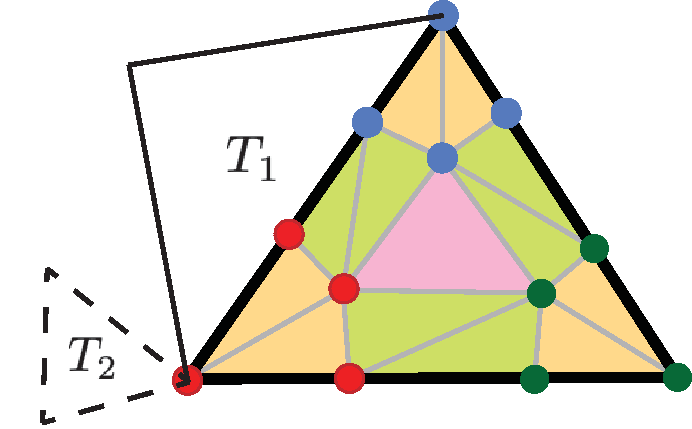
\includegraphics[width=0.5\linewidth]{prism-tex/figs/bevel_colors}
    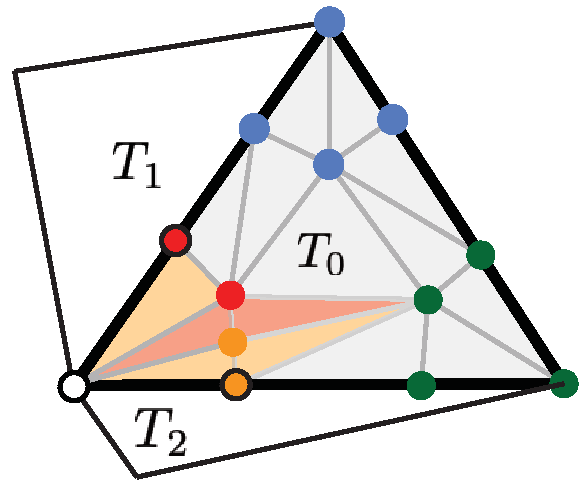
\includegraphics[width=0.4\linewidth]{prism-tex/figs/singularity-bevel-explained}
    \caption{Bevel patterns used in the proofs in Appendix~\ref{app:bevel} and Appendix~\ref{app:singularity}}
    
    \label{prism:fig:bevel-explain}
    \vspace{-1em}
\end{figure}
% The prism on the pink... \DZ{incomplete sentence}
The prism {corresponding to} the {pink} triangle covers only the interior of the original triangle. It satisfies {the dot product condition} since {its pillars are copied from the solution of Problem~(\ref{eq:QP})} at each vertex. 
A similar argument can be made for the green {prisms}: each  {prism} 
{gets its pillars from the edges}
incident at two of the vertices, {which are compatible with the normal of the adjacent triangle (e.g., red and blue pillars have positive dot product with  {the normal of} $T_1$).}
%Since the green triangles cover exactly the two triangles in the 1-ring of both vertices, it also satisfies I2. 
Finally, the prisms corresponding to orange triangles cover the same one ring that was used to compute the {original pillars (e.g., red pillar is compatible with $T_1$ and $T_2$)}. Since the same {pillar} is used for  each of the 3 vertices of the original prism, {the dot product} is {unchanged}.

\subsection{Theorem \ref{thm:invariants}}\label{app:invariant-checks}
% \begin{proof}
We use $A^\circ$ to denote the interior of a set $A$. 
We first assert that the topological disk patch $\T \cap C$ coincides with $\T \cap C'$.
%\DZ{there is a slight abuse of notation here: }
%$\T$ \DZ{is a collection of faces, and here the reference is to the geometry defined by these faces; one way to deal with this is to use 
%something like} $|\T|$ \DZ{for the point set defined by the mesh}
To make the notation more concise, we define $\T_C = \T \cap C$ and $\T_{C'} = \T \cap C'$.

We show that $\T_C \subset C'$ by contradiction: assume there is $p\in \T_C$ but $p \not\in C'$.
Choose a point $q \in \partial \T_C$,  that belongs to single prisms in $C$ and $C'$ and denote the enclosing prism in $C$ as $\Prism_q$ and the corresponding one in $C'$ as $\Prism_{q}'$.
It follows from the positivity of the volumes of $\Prism_q$ and $\Prism_q'$ (Assumption 1), that there is  $\varepsilon>0$ such that the half-ball (for sufficiently small $\varepsilon$)  $\text{Ball}(q, \varepsilon) \cap \Prism_q$  coincides with $ \text{Ball}(q, \varepsilon) \cap \Prism_q'$.
Futhermore, the validity of the initial shell guarantees that there exists an interior point $\bar{q} \in \text{Ball}(q, \varepsilon) \cap \Prism_q^\circ \cap \T$, and $\bar{q}\in \Prism_q'^\circ \cap \T \subset C'^\circ\cap \T$.

 Since neither $p$ or $\bar{q}$ lies on the boundary side triangles of $\partial C'$ (since $p,\bar{q}\notin\partial \T_C$), therefore there exists an interior path $P$ (i.e., a path both in $\T_C$ and in $\T_{C'}$) that connects $p$ and $\bar{q}$. By continuity the path $P$ it will cross $\partial C'$ at some point $p_i\in \T_C$. 
Since the $\partial \T_{C'} = \partial \T_C$ is a fixed boundary loop (by the definition of $\mathbb{O}$), and does not contain interior points, $p_i$ can only cross on the top surface or bottom surface of $C'$ which contradicts Assumption 2. The roles of $C$ and $C'$ can be inverted to complete the proof. 

We then  map $M_C$ to a
regular planar $n$-gon $D$, with vertices on $\partial M_C$ mapped cyclically to the vertices of $\partial D$.
It follows from \cite[Corollary 6.2]{floater2003one} that such a convex combination mapping $\varphi\colon M_C \to D$ is bijective. Then, similarly to the construction in Theorem~\ref{thm:projection},
we 
%``lift'' $D$ and 
define $\phi\colon C \to D\times[-1,1]$ through affine mapping induced by the thetrahedralization of the prisms $\Prism_i$.
%
Similarly, we define $\psi \colon C' \to D\times[-1,1]$. The mapping $\psi$ is also bijective because of Assumption 1 and the definition of $\mathbb{O}$ it follows that the codomain of $\psi$ is the same as $\phi$.
%
Note that in both cases, the map transforms the vector field $\V(p)$ to the constant vector field $e_z = (0,0,2)$, and the projection is $\P_z$, as defined in Appendix~\ref{app:projection}. 

The dot product condition (Assumption 3) ensures that $\P_z$ defines a bijection between $D$ and $\psi(\T_C)$\revision{;} and further, the image \revision{satisfies} $\P_z(\psi(\Prism_i'\cap \T)) = \psi(M_i')$ where $M_i'$ is the middle surface (a single triangle) of $\Prism_i'$.
Therefore, since $\psi$ and $\P_z$ are both continuous and bijective, they are homeomorphisms which preserve topology, 
thus $\Prism_i'\cap \T $ is a simply connected topological disk.
% \end{proof}


\section{Extension to meshes with Singularities}\label{app:singularity}
Most of the proofs and definition in Section~\ref{prism:sec:method} easily extends to meshes with singularity or pinched shells. For instance,
\revision{both} Theorem~\ref{thm:projection} and Definition~\ref{def:validshell} apply to pinched shells by just considering a prism made of 4 (2 for the top and 2 for the bottom slab) instead of 6. Propositions~\ref{thm:I1} and~\ref{thm:thickness} both rely on per-vertex properties; by just excluding singular vertices (and neighboring prism) from the statements the proofs (and our algorithm) still holds.


Theorem~\ref{thm:invariants} requires some minor additional considerations. As a consequence of beveling, no two singularities are adjacent. Therefore, we can always find a point $q \in \partial \T_C$ that belongs to a single prism (Appendix~\ref{app:invariant-checks}) since every prism will have a positive volume
because no singularities are adjacent.


Finally Proposition~\ref{thm:bevel} requires a new proof since the beveling pattern used for singularities is different.
% \begin{proposition}
% For a prism $\Prism$ with one singularity, 
% \end{proposition}
\begin{proof}
In  Figure~\ref{prism:fig:bevel-explain} right, we highlight in red and orange the triangles not covered by the discussion in Appendix~\ref{app:bevel}. 
The prism corresponding to an orange middle triangle intersects the edge-adjacent triangle. And since the new pillars are computed as the average of the normals of the two adjacent triangles with dihedral angle strictly less than $360^\circ$ 
 (Section~\ref{prism:sec:singularities} inset), each dot product is positive. 
The prism \revision{for} a pink middle triangle intersects only the interior of the original triangle, and the dot product between the pillars and the triangle normal are positive by construction. %\DZ{compatible?}
\end{proof}



\section{Reduction to a Standard QP}
\label{app:qp}

With slack variable $t$, Problem \ref{eq:OPT} can be rewritten as

$$\max_t t;\; d_v n_f \geq t, \|d_v\| = 1, t \geq {\epsilon}.$$

In the admissible region, substituting $t = 1/s$, 
$$\min_s s;\; s d_v n_f \geq 1, \|d_v\| = 1, {0< s \leq 1/\epsilon}.$$
Substituting $x=s d_v$ (thus $\|x\| = s\|d\| = s$), we obtain the QP problem \ref{eq:QP}. Note that the lower bound on $s$ is implied from $s d_v n_f \geq 1$, and the upper bound $\|x\| < 1/\epsilon$ is checked a posteriori.

%   convex.  The objective is convex, because we can write it as linear inequality constraints $d_v \cdot n_f \geq t$, and the objective is simply $t$.
% }
% \DZ{ Continuing the remark above, consider the problem in a (more) standard form, i.e. 
% $\max t,\;  d_v \cdot n_f > t,\;  d_v \cdot n_f > 0,\; \| d_v \| \leq 1$. We can replace the constraints 
% $d_v \cdot n_f > 0$ with a single constraint $t > 0$.  Furthermore, replacing $t$ with $s^2$, 
% we eliminate the need for that constraint entirely; the probem becomes  $\max s^2,\; d_v \cdot n_f > s^2, \| d_v \| \leq 1$.  Define $x = d_v/s$,  then the problem is $\min \|x \|^2, x \cdot n_f >  1, \| x s \| \leq 1$. As $s$ does not  enter any other equation in the problem, it can always be used to satisfy the last inequality; thus we obtain the equivalent problem \eqref{eq:QP}.  This proves equivalence.  However, as the orignal problem was immediately equivalent to a QP in the first place, there is no point}
%

\section{Bijectivity of the Nonlinear Prismatic Transformation}
\label{app:bilinear}
In this section, we show
that the isoparametric transformation of prismatic finite element \cite{ciarlet1991basic} is also bijective if I1 holds.%(on each half of the shell).

We follow the notation from {Appendix~\ref{app:I1}.} 
The map is defined as (for the top slab)
\begin{align*}
    f(u,v,\eta) &= u e_1 + v e_2  + \eta n_0 + u \eta \revision{n_{01}} +
    v \eta \revision{n_{02}},\\
    \det J_f &=  \langle (1-u-v) n_0 + u n_1 + v n_2, e_1 + \eta \revision{n_{01}},
    e_2 + \eta \revision{n_{02} \rangle,}
\end{align*}
where $\eta$ is the variable corresponding to the thickness direction\revision{, and $n_{ij} = n_j - n_i$.}
Observe that $\det J_f(u,v,\eta_0)$ is linear in $u,v$ for fixed $\eta_0$, the extrema will only be achieved at the corner points \cite{knabner2001invertibility}. Therefore, it is sufficient to check the signs at three edges
$(0,0,\eta)$, $(1,0,\eta)$, $(0,1,\eta)$ for $\eta \in [0,1]$.
\begin{align*}
    & \det J_f(0,0,\eta) \\
    &= \langle n_0, (1-\eta)e_1 +\eta (e_1 + n_1 - n_0),(1-\eta)e_2 +\eta (e_2 + n_2 - n_0) \rangle \\
    &= (1-\eta)^2\langle n_0, e_1, e_2 \rangle + 
    (1-\eta)\eta \langle n_0,e_1, e_2+n_2\rangle \\&+ 
    (1-\eta)\eta \langle n_0, e_1+n_1, e_2\rangle + 
    \eta^2\langle n_0, e_1+n_1, e_2 + n_2\rangle\\
    &= (1-\eta)^2 \text{vol}_4 + (1-\eta)\eta (\text{vol}_3 +\text{vol}_1) + \eta^2 \text{vol}_2 > 0.
\end{align*}

By symmetry, 
it is easy to verify \revision{that the following are positive},
\begin{align*}
    \det& J_f(1,0,\eta) = (1-\eta)^2 \text{vol}_6 + (1-\eta)\eta (\text{vol}_7 +\text{vol}_5) + \eta^2 \text{vol}_8\revision{,} \\
    \det& J_f(0,1,\eta) = (1-\eta)^2 \text{vol}_{11} + (1-\eta)\eta (\text{vol}_9 +\text{vol}_{10}) + \eta^2 \text{vol}_{12}.\\
\end{align*}


\section{Double Slab}\label{app:dblayer}
In Section~\ref{prism:sec:projection}, we explain that we want to ensure that our shell validity is independent from the enumeration of the faces; for this reason, we require that the conditions I1 and I2 are satisfied for all possible decompositions. Without using the double slab, different decompositions of the prism will result in  different intersections with the middle surface. In other words, the projection operator will project the input mesh to a different set of triangles on the middle surface. 
The double slab makes the middle surface independent of the decomposition by construction. 
We note that Theorem~\ref{thm:bevel} is valid only for double-slab prisms since the statement requires that one prism contains only one triangle.

\section{Unpublished Material}
(Disclaimer: this section is unpublished material. And serves as post publish notes for future references.)
\subsection{Pointless Variant}
We extend the framework, by allowing the relaxation of definition of a section. 
Originally, any intersection between the triangle and the (different decomposition of the) prism is counted. Here, we explicitly forgive when the intersection is only one point on the vertex of mid surface and the triangle. 
This predicate can be easily implemented, making use of the bitwise equal coordinates.
Therefore, the initial tracking section only follows edge-adjacency relationship, instead of the vertex adjacent one in the main text. 
With such adjusted condition for section, the optimization can be trivially accomodated. The only thing that is different (simpler) is the part for bevel, since we have less triangles to consider.
The existing one is still valid, however, we can get away with simpler red-green intersection

\subsection{Dynamic Intersection Check}
To make easier the guarantee of a self-intersection-free shell, substitue the AABB tree collision check with a dynamic hashgrid. We initialize two hashgrids at the beginning, one for top surface and another one for bottom surface. This is followed by additional shrinking to make sure they are clear. Each local opeartion is responsible to trial and keep the validity of the surfaces. Furthermore, the top/bottom surface should not interfere with the reference input surface, this can be accelerated through the maintainance of the tracking list, and is trial checked before a local operation is performed.

\subsection{Feature Snapping Shell}
We can separate the definiition of reference surface and input surface to make a feature snapping shell.

\subsection{Positive Detereminant for Natural Prism Map}
This section follows and extends Appendix~\ref{app:bilinear}
In fact, we observe that, for a quadratic bezier curve piece $a t^2 + b t (1-t) + c (1-t)^2, t\in [0,1]$, the sufficient and necessary condition is $a>0, c>0, b > - 2 \sqrt{a c}$, and the last relation is equivalent to (but more clearly stated as) $b > 0 || b^2 - 4 a c < 0$.
The current text (all 12 positive tetra) impose an unnatural constraint on edge splits: in the case of an agressively positive prism (all decompositions are all-positive), sub-prism may not be positive in the same sense. While this will not break anything, forbidding edge split will lead to unexpected lower quality in the optimization procedure.
